\section{Damara Benedicta}
\subsection{Sejarah}
Python merupakan suatau bahasa pemrograman skrip yang tidak sulit untuk dibaca dan ditulis, dan tidak memiliki fungsi yang terbatas sehingga dapat digunakan untuk menyelesaikan berbagai macam tugas
Python awal mula dikembangkan tahun 1990 oleh guido van Rossum di Amsterdam. Nama python berasal dari nama yang dipilih oleh guido dari acara televisi sirkus monty pyton.
Pada 1995 versi yang dirilis oleh CWI adalah versi 1.2. dan versi terakhir pada tahun 2000 adalah versi 1.6. dan python 2.0 mulai dirilis oleh BeOpen. Setelah menghapus Python 2.0, Guido dan anggota tim PythonLabs lainnya pindah ke DigitalCreations. Distribusi Python telah mencapai versi 2.6.1 dan versi 3.0, dan dengan demikian mencegah Python dimiliki oleh perusahaan komersial. Saat ini distribusi Python telah mencapai versi 2.7.14 dan versi 3.6.3
\subsection{Instalasi Anaconda}
\begin{enumerate}
    \item Pastikan Bahwa Python telah terinstal dilaptop anda.
    \item Jika anda belum punya anaconda, kalian bisa download di https://www.anaconda.com/distribution/#download-section
    \item Kemudian buka installer yang telah di download barusan
    \item Klik next
    \begin{figure}[!htbp]
        \centering
        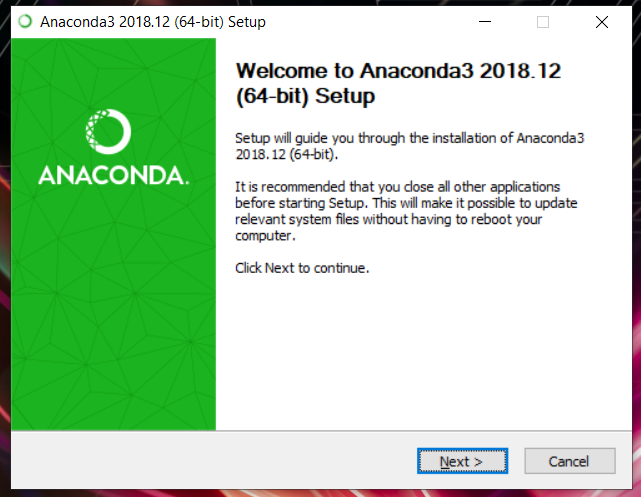
\includegraphics[width=3cm,height=3cm]{figures/1.png}
        \caption{Tampilan Awal}
        \label{awal}
        \end{figure}

    \item Kemudian Klik Next
    \begin{figure}[!htbp]
        \centering
        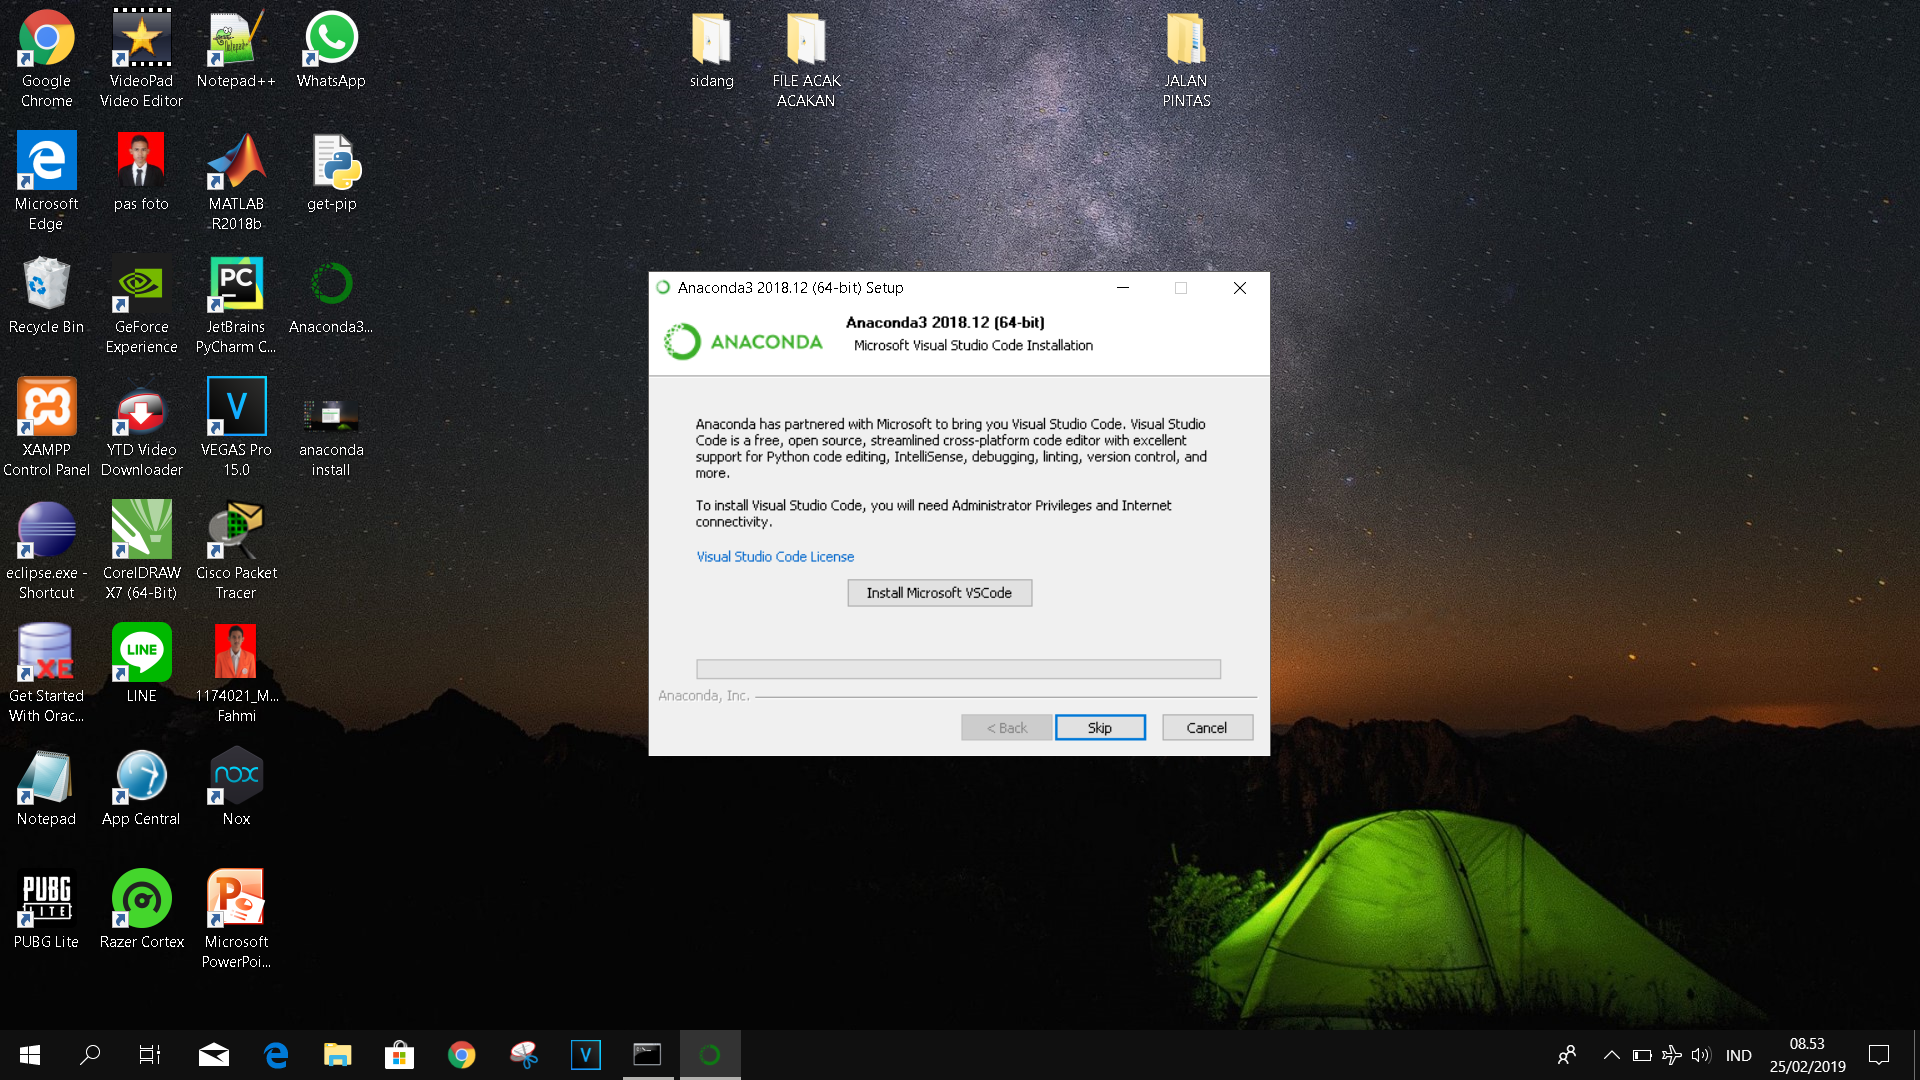
\includegraphics[width=3cm,height=3cm]{figures/2.png}
        \caption{License Agreement}
        \label{License}
        \end{figure}

    \item Kemudian akan muncul persetujuab lisensi, setelah itu pilih " I Agree"
    \begin{figure}[!htbp]
        \centering
        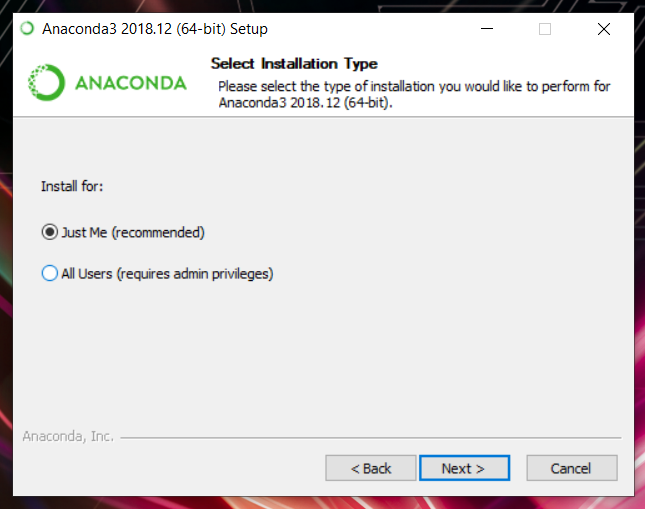
\includegraphics[width=3cm,height=3cm]{figures/3.png}
        \caption{Pemilihan User}
        \label{User}
        \end{figure}

    \item Kemudian memilih tipe instalasi
    \begin{figure}[!htbp]
        \centering
        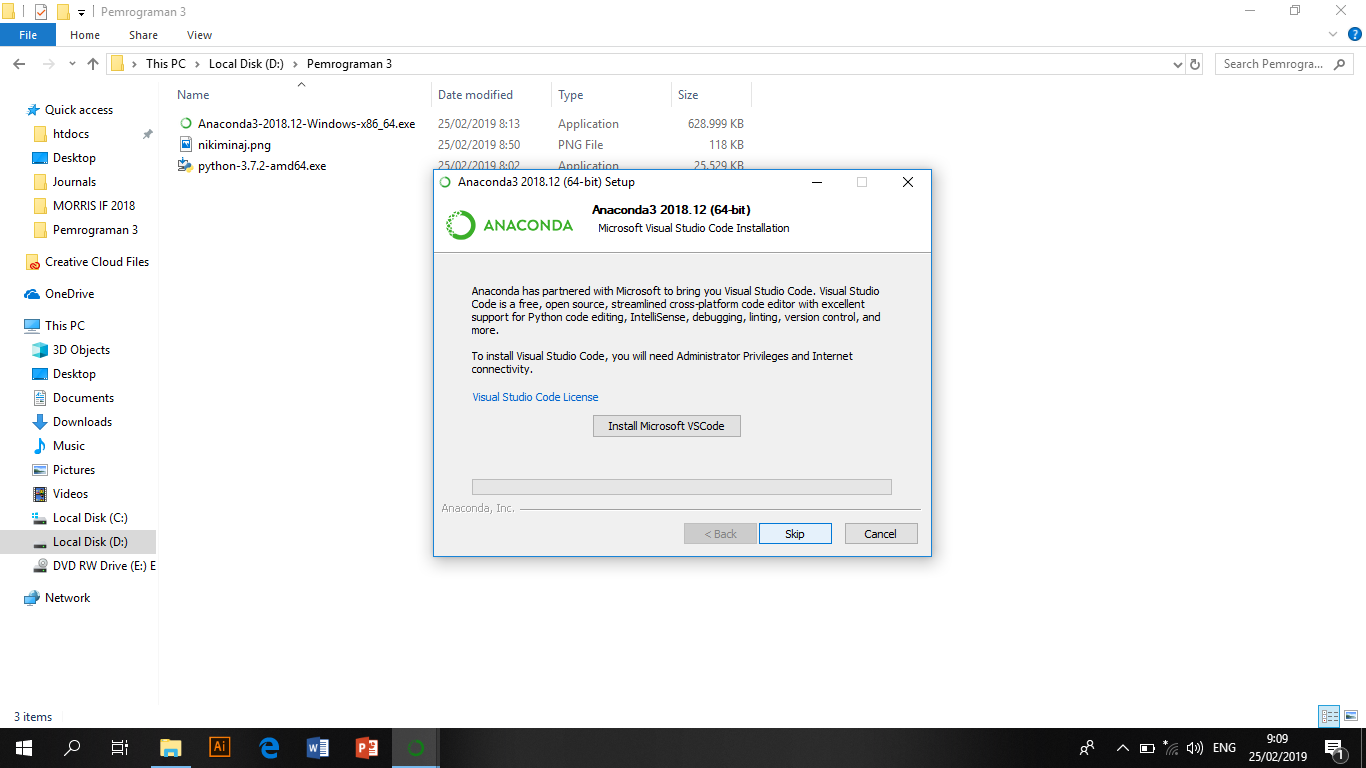
\includegraphics[width=3cm,height=3cm]{figures/4.png}
        \caption{Pemilihan Direktori Penyimpanan}
        \label{Directory}
        \end{figure}

    \item Kemudian pilih lokasi untuk instal, setelah itu klik Next
    \begin{figure}[!htbp]
        \centering
        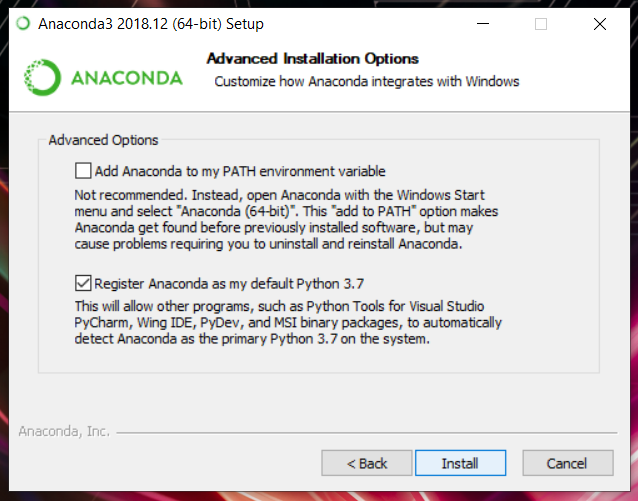
\includegraphics[width=3cm,height=3cm]{figures/5.jpeg}
        \caption{Pemilihan Opsi}
        \label{opsi}
        \end{figure}

    \item Kemudian centang pada kotak register dan pilih instal
    \begin{figure}[!htbp]
        \centering
        \includegraphics[width=3cm,height=3cm]{figures/6).png}
        \caption{Proses Instal}
        \label{Proses}
        \end{figure}

    \item Kemudian Klik next
    \begin{figure}[!htbp]
        \centering
        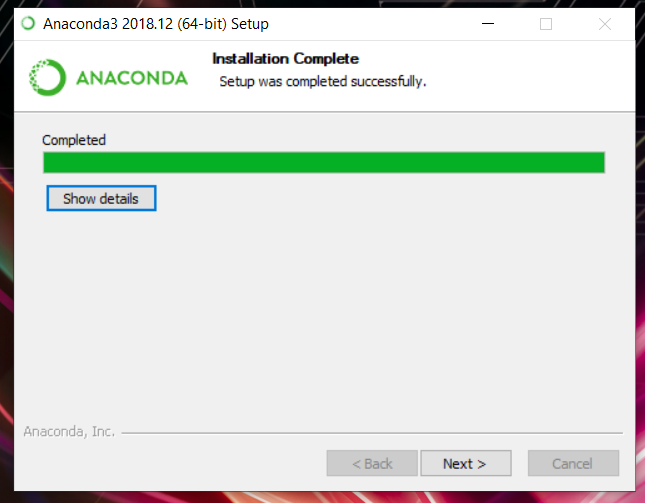
\includegraphics[width=3cm,height=3cm]{figures/7.png}
        \caption{Proses Instal Selesai}
        \label{Proses}
        \end{figure}

    \item kemudian jika tidak akan mengistal VSCode, maka pilih skip
    \begin{figure}[!htbp]
        \centering
        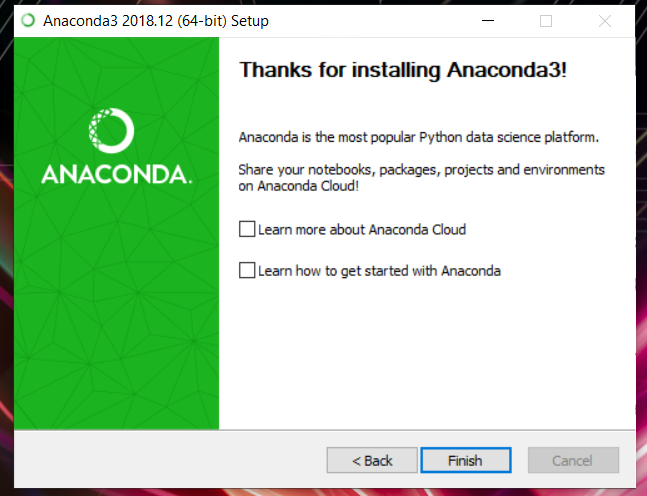
\includegraphics[width=3cm,height=3cm]{figures/9.png}
        \caption{Penawaran Instal MS VSC}
        \label{offering}
        \end{figure}
        \item kemudian Proses intalasi telah selesai pilih finish
    \begin{figure}[!htbp]
        \centering
        \includegraphics[width=3cm,height=3cm]{figures/12.png}
        \caption{Penawaran Instal MS VSC}
        \label{offering}
        \end{figure}
\end{enumerate}
\subsection(Spyder)
Spyder adalah tools yang dipakai untuk python 
    \begin{figure}[!htbp]
        \centering
        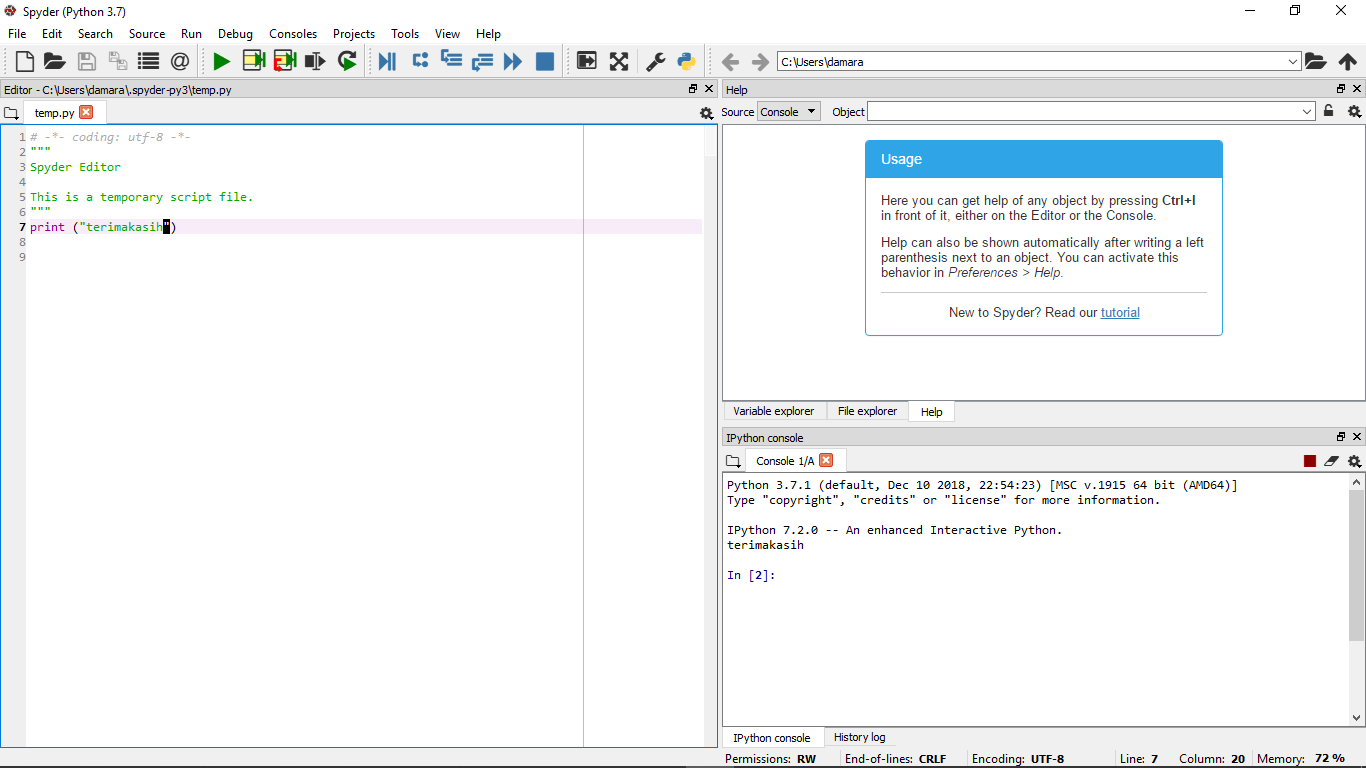
\includegraphics[width=3cm,height=3cm]{figures/Screenshot(1).png}
        \caption{Instalasi Selesai}
        \label{akhir}
        \end{figure}


